%
% Copyright (C) 2004-2009 Jason Blevins <jrblevin@sdf.lonestar.org>
% http://jblevins.org/projects/cv-template/
%
% You may use use this document as a template to create your own CV
% and you may redistribute the source code freely. No attribution is
% required in any resulting documents. I do ask that you please leave
% this notice and the above URL in the source code if you choose to
% redistribute this file.

\documentclass[letterpaper, 10pt]{article}

\usepackage{hyperref}
\usepackage{geometry}
\usepackage[minbibnames=4,maxbibnames=4,sorting=ydnt,date=comp,isbn=false,doi=false]{biblatex}
\addbibresource{papers.bib}

\AtEveryBibitem{%
	\clearfield{note}%
}

\DeclareSortingTemplate{ndymdt}{
	\sort[direction=descending]{
		\field{sortyear}
		\field{year}
		\literal{9999}
	}
	\sort[direction=descending]{
		\field[padside=left,padwidth=2,padchar=0]{month}
		\literal{99}
	}
	\sort[direction=descending]{
		\field[padside=left,padwidth=2,padchar=0]{day}
		\literal{99}
	}
	\sort{
		\field{presort}
	}
	\sort[final]{
		\field{sortkey}
	}
	\sort{
		\field{sortname}
		\field{author}
		\field{editor}
		\field{translator}
		\field{sorttitle}
		\field{title}
	}
	\sort{
		\field{sorttitle}
	}
	\sort[direction=descending]{
		\field[padside=left,padwidth=4,padchar=0]{volume}
		\literal{9999}
	}
}

\usepackage{graphicx}
\usepackage{enumitem}

%\usepackage[sfdefault]{cabin}
%\usepackage[T1]{fontenc}

%\usepackage[sfdefault]{overlock} %% Option 'sfdefault' only if the base font of the document is to be sans serif
\usepackage[default,oldstyle,scale=0.95]{opensans}
\usepackage[T1]{fontenc}



% Set your name here
\def\name{George G. Vega Yon}

% Replace this with a link to your CV if you like, or set it empty
% (as in \def\footerlink{}) to remove the link in the footer:
\def\footerlink{https://ggvy.cl}

% The following metadata will show up in the PDF properties
\hypersetup{
  colorlinks = true,
  urlcolor = blue,
  pdfauthor = {\name},
  pdfkeywords = {economics, statistics, mathematics},
  pdftitle = {\name: Curriculum Vitae},
  pdfsubject = {Curriculum Vitae},
  pdfpagemode = UseNone
}

\geometry{
%  body={6.5in, 9in},
  left=1.3cm,
  top=1in,
  right=1.3cm,
  bottom=1in
}

% Customize page headers
\usepackage{fancyhdr}
%\pagestyle{myheadings}
%\markright{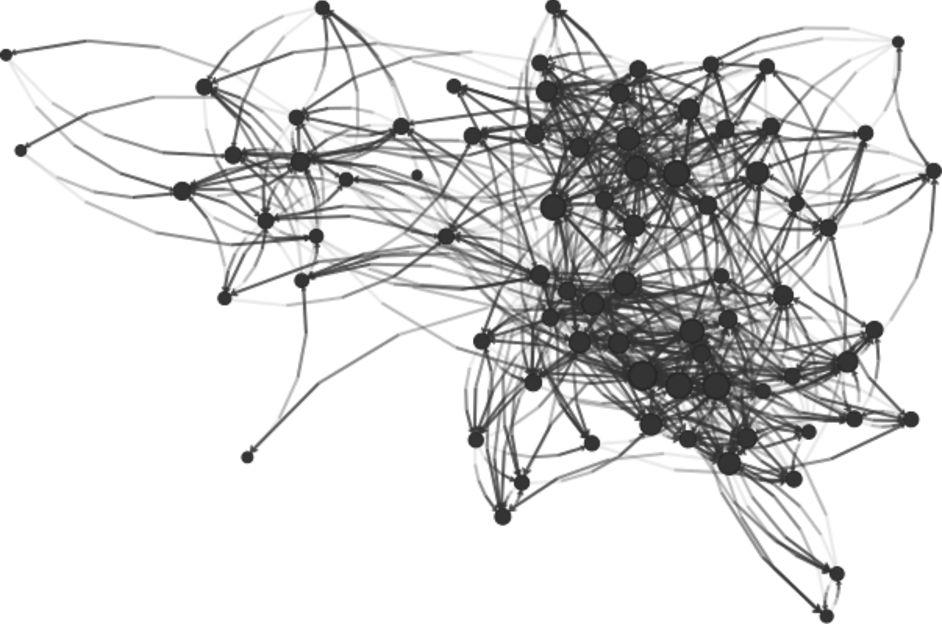
\includegraphics[width=1cm]{fig/ukfaculty.pdf} \name}
\pagestyle{fancy}
\fancyhead{}
\fancyfoot{}
\renewcommand{\headrulewidth}{0pt}
\fancyhead[L]{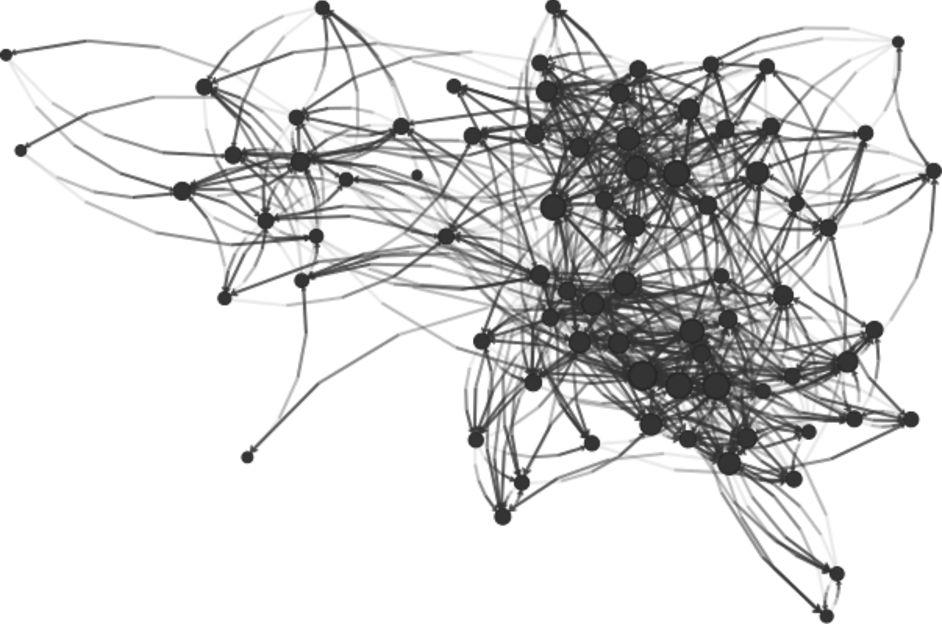
\includegraphics[width=1cm]{fig/ukfaculty.pdf}\\\vspace{-.75cm}\hspace{1.1cm}\emph{\name}}
\fancyhead[R]{\small\thepage}
\thispagestyle{empty}

% Custom section fonts
%\usepackage{sectsty}
%\sectionfont{\sffamily\mdseries\Large}
%\subsectionfont{\sffamily\mdseries\itshape\large}

% Other possible font commands include:
% rmfamily
% \ttfamily for teletype,
% \sffamily for sans serif,
% \bfseries for bold,
% \scshape for small caps,
% \normalsize, \large, \Large, \LARGE sizes.

% Don't indent paragraphs.
\setlength\parindent{0em}

% Make lists without bullets
\renewenvironment{itemize}{
  \begin{list}{}{
    \setlength{\leftmargin}{0.45cm}
  }
}{
  \end{list}
}

% Para poder poner comandos genericos en tablas (en el inicio del argumento)
\usepackage{array}

\renewcommand{\bf}{\bfseries\color{teal}}
\renewcommand{\textbf}[1]{{\bfseries\color{teal}#1}}
\usepackage{xcolor}
\begin{document}
	
	% Place name at left
	\hfill 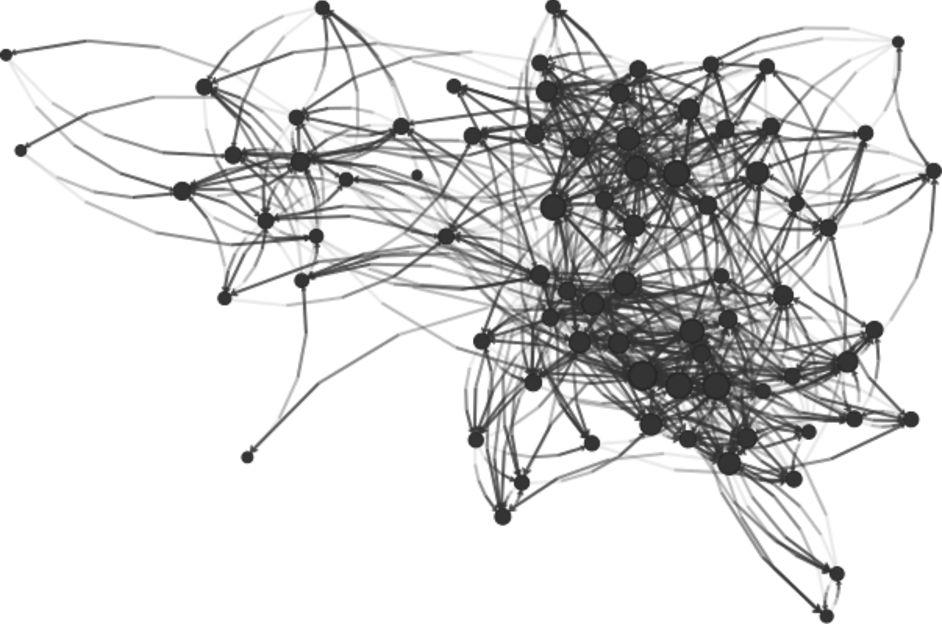
\includegraphics[width=.4\linewidth]{fig/ukfaculty.pdf}\vspace{-6cm}
	\part*{\color{darkgray}{\name}}



% Alternatively, print name centered and bold:
%\centerline{\huge \bf \name}

%\vspace{0.25in}

\begin{minipage}{0.50\linewidth}
  \begin{tabular}{>{\bfseries}p{.2\linewidth}p{.79\linewidth}}
    Mobile & +1 (six two six) 381 8171 \\
    e-mail & \href{mailto:g.vegayon@gmail.com}{\tt g.vegayon@gmail.com} \\
    website & \href{https://ggvy.cl}{\tt ggvy.cl} \\
    Code & \href{https://github.com/gvegayon}{\tt github.com/gvegayon}\\
    Linkedin & \href{https://www.linkedin.com/in/georgevegayon/}{\tt www.linkedin.com/in/georgevegayon/} %\\
    %Talks & \href{https://ggv.cl/talk}{\tt ggv.cl/talk}
  \end{tabular}
\end{minipage}


\section*{Education}

\begin{itemize}
\item 
{\bf Ph.D. in Biostatistics (concentration in Stat. Comp.)} University of Southern California (2020). Dissertation \emph{``Essays on Bioinformatics and Social Network Analysis: Statistical and Computational Methods for Complex Systems''}

{\bf M.Sc. in Social Sciences (Economics)} California Institute of Technology (2016)

{\bf Master in Economics and Public Policy}, Universidad Adolfo Ib\'a\~nez (2011)

{\bf BS. in Social Sciences} and {\bf BS. in Business Administration}, Universidad Adolfo Ib\'a\~nez (2011)
\end{itemize}

\section*{Professional Experience}

\begin{itemize}
\item \textbf{University of Utah, November 2021--Present} Division of Epidemiology \emph{Research Assistant Professor}.
\item \textbf{University of Southern California, 2015--November 2021} Department of Preventive Medicine \emph{Research Programmer}. As a senior research staff member, my responsibilities include: Provide technical support on statistical computing, e.g., HPC, run training sessions on scientific software development, and writing scientific papers. Since August 2020, I co-instruct the Department's Introduction to Data Science class.
\item \textbf{Chilean Pension Supervisor, August 2011-- August 2014} Research Division \emph{Analyst}. Statistical and econometric analysis on the Chilean unemployment insurance, statistical software development, serving as a bridge between the IT and Research divisions.
\item \textbf{Nodos Chile Social Network Analysis Ltda., January 2012--January 2014} \emph{Partner}.
Founding partner of one of the first applied SNA Consultancy Entrepreneurship in Chile.
\item \textbf{Universidad Adolfo Ib\'a\~nez, January 2011--June 2012.} School of Government \emph{Adjunct Professor}.
Taught Introductory courses of Economics, Microeconomics and Statistical computing with Stata.
\item \textbf{Chilean Ministry of Social Planning, March 2011--December 2011.} Social Programs Monitoring \emph{Analyst}.
Survey and Analysis of the Government social programs supply and supporting the Monitoring Division with the Open-Data Initiative.
\end{itemize}

\section*{Software {\small (selected)}}

\begin{enumerate}[label={[}\arabic*{]},labelindent=5\parindent,labelsep=8pt]
\item {\bfseries George G.} {\bfseries Vega Yon}. \textit{{aphylo: Statistical Inference of Annotated Phylogenetic Trees}} (2022). R package version 0.2-1 {\small URL}: \url{https://cran.r-project.org/package=aphylo}. 
\includegraphics[width=2.5cm]{fig/cran-downloads-rgexf.pdf}
\item {\bfseries George G.} {\bfseries Vega Yon}. \textit{rgexf: Build, Import and Export GEXF Graph Files} (2020). R package version 0.16.0. {\small URL}: \url{https://CRAN.R-project.org/package=rgexf}. 
\includegraphics[width=2.5cm]{fig/cran-downloads-rgexf.pdf} 
\item {\bfseries George G.} {\bfseries Vega Yon}, Thomas Valente. \textit{{{netdiffuseR: Analysis of Diffusion and Contagion Processes on Networks}}} (2020). R package version 1.22.0. {\small URL}: \url{https://github.com/USCCANA/netdiffuseR}. 
\includegraphics[width=2.5cm]{fig/cran-downloads-netdiffuser.pdf} 
\item {\bfseries George G.} {\bfseries Vega Yon}, Kayla de la Haye. \textit{ergmito: Exponential Random Graph Models for Small Networks} (2020). R package version 0.3-0. {\small URL}: \url{https://cran.r-project.org/package=ergmito}. 
\includegraphics[width=2.5cm]{fig/cran-downloads-ergmito.pdf} 
\item {\bfseries George G.} {\bfseries Vega Yon}. \textit{slurmR: A Lightweight Wrapper for 'Slurm'} (2020). R package version 0.4-1. {\small URL}: \url{https://CRAN.R-project.org/package=slurmR}. 
\includegraphics[width=2.5cm]{fig/cran-downloads-slurmr.pdf} 
\item {\bfseries George G.} {\bfseries Vega Yon}. \textit{fmcmc: A friendly MCMC framework} (2020). R package version 0.3-0. {\small URL}: \url{https://CRAN.R-project.org/package=fmcmc}. 
\includegraphics[width=2.5cm]{fig/cran-downloads-fmcmc.pdf} 
%\item {\bfseries George G.} {\bfseries Vega Yon}. \textit{barry: your to-go motif accountant} (2020). C++ library version 0.0-1. {\small URL}: \url{https://github.com/USCbiostats/barry}.  
\end{enumerate}

\section*{Academic Publications {\small (selected)}}

\nocite{yon2019exponential,VegaYon2019c,VegaYon2019a,vegayon2020aphylo,Hancean2022,ouellet2022} %VegaYon2019b

\printbibliography[title=\vskip-20pt,omitnumbers=true]



%\subsection*{Conferences and Presentations}
%
%\begin{itemize}
%\item ``PARALLEL: Stata module for parallel computing'', presented at the {\it Stata Conference} (2013), New Orleans, USA.
%\item ``Introducing {\tt rgexf} and how to develop your own R-package'', presetented at the {\it Group of R users in Chile} (2013), Santiago, Chile.
%\item ``Introducing PARALLEL: Stata Module for Parallel Computing'', presented at the {\it Reuni\'on Anual de la Sociedad de Economistas de Chile} (2012), Vi\~na del Mar, Chile.
%\end{itemize}

%\subsection*{Press and others}
%
% \begin{itemize}
%\item
%\href{https://gephi.wordpress.com/2013/02/12/rgexf-an-r-library-to-work-with-gexf-graph-files/}{``rgexf: An R library to work with GEXF graph files''} in {\it Gephi Blog}, published in february 12, 2013.
%\item \href{http://www.elmostrador.cl/opinion/2012/04/04/aborto-en-twitter-un-debate-a-medias/}{``Aborto en Twitter: un debate a medias''} in {\it El Mostrador}, published in april 4, 2012.
%\item \href{http://www.uai.cl/200911165701/columna-de-opinion/columnas-opinion/reinventar-la-ciudadania-la-otra-campana-que-obama-esta-ganando}{``Reinventar la ciudadanía, la otra campaña que Obama está ganando''} in {\it El Mostrador}, published in november 10, 2009.
%\end{itemize}

\section*{Honors and Professional Achievements}

\begin{itemize}
\item \textbf{Technologies} R, C++, \LaTeX, SQL, python, XML, regex, Stata, VBA, Gephi, Pajek, Mathematica, git, Docker, Visual Studio Code, unix.
\item \textbf{Book reviewer}: ``Microeconometrics and Matlab: An Introduction'', by Adams, Clarke and Quinn, Oxford University Press, 2015. ``Mastering Gephi Network Visualization'', by Ken Cherven, Packt Publishing, 2015. ``Network Graph Analysis and Visualization with Gephi'', by Ken Cherven, Packt Publishing, 2013.
\item \textbf{Awards} Travel Grant, Society of Young Network Scientist, 2019; Fellowship, California Institute of Technology, 2014; Scholarship, Adolfo Ib\'a\~nes University, 2006.
%\item \textbf{Book reviewer} ``Microeconometrics and MATLAB'', by Abi Adams, Damian Clarke \& Simon Quinn, Oxford University Press, (forthcoming 2015).
\item \textbf{Manuscript reviewer} The Official Journal of The Society for Computational Economics, The R Journal, Social Networks, Journal of Mathematical Sociology, Journal of Open Source Software, Bioinformatics, Computer Methods and Programs in Biomedicine Update, American Statistical Association, SUNBELT Conference (2016), International Conference on Computational Social Science (2019--2021).
\item \textbf{Misc} Founder of the \href{https://www.meetup.com/useRchile/}{R Users Group in Chile (2013)}, co-organizer of the \href{https://socalr.org}{East LA R User Group (LAERUG)}.
%\item \textbf{Honorable Mention} (Posters Sesion. Work: \emph{Introducing Parallel: Stata Module for Parallel Computing}) given by the Chilean Economics Society during its 2012 annual meetting.
%\item \textbf{Honour Scholarship} given by Adolfo Ib\'a\~nez University for completing undergrad and graduate studies (2006-2010).
%\item \textbf{Software workshop, 2010.} \emph{Co-founder} of the workshop thaught by Economics and PP Masters's Students at Adolfo Ib\'a\~nez University in order to introduce grad students into scholar research software (\LaTeX, \emph{R}, Stata, etc.).
\end{itemize}

\bigskip

% Footer
\begin{center}
 \begin{footnotesize}
   last update: \today \\
   \href{\footerlink}{\texttt{\footerlink}}
 \end{footnotesize}
\end{center}

\end{document}

